\begin{frame}{Goals for Honeycomb Mott Insulator}
\vskip-1.5cm
\bi 
\item Build a tensor network representation for doing computations
\item <1-> Verify that no spontaneous symmetry breaking occurs
%We'll do this by computing correlation functions on a cylinder geometry combined with scaling analysis in the circumference

\only<1>{
\begin{figure}
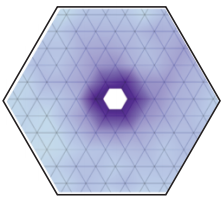
\includegraphics[width=6cm]{diagrams/kimchicorr.png}
\caption{Exponentially decaying rotationally symmetric correlations computed using Monte Carlo sampling, \citep{Kimchi2012-lr}}
\end{figure}
}

\only<2->{
\begin{figure}
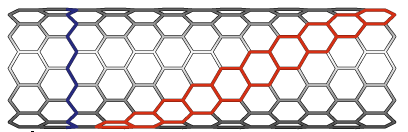
\includegraphics[width=6cm]{diagrams/Zig.png}
\end{figure}

\item<3-> Rule out topological order

\item<4-> Compute entanglement spectrum to check for nontrivial entanglement
\item<5-> Understand the role of symmetries in protecting entanglement in interacting quasi-1D and 2D theories
\item<6-> Find distinguishing topological invariant and/or physical signatures
\item<7-> Find a parent Hamiltonian 
%then you can do things like perturb hamiltonian to show that it is a stable phase if certain symmetries are kept, and drive phase transitions to lattice SB insulators or superfluids.
% also you can dope it and make a superfluid with some properties.

}
\ei 
\end{frame}